%%%%%%%%%%%%%%%%%%%%%%%%%%%%%%%%%%%%%%%%%%%%%%%%%%%%%%%%%%%%%%%%%%%%%%%%%%%%%%%%%%
\begin{frame}[fragile]\frametitle{}
\begin{center}
{\Large Notes from Teachings of Krishna Prakash of Shrimath}
\end{center}
\end{frame}

%%%%%%%%%%%%%%%%%%%%%%%%%%%%%%%%%%%%%%%%%%%%%%%%%%%%%%%%%%%
\begin{frame}[fragile]\frametitle{Starting Yoga}

	\begin{itemize}
	\item Yoga Sadhna is An Endless Ocean	
	\item You cannot be a Yoga Teacher/Guru just after training or certification, practice it for years (12), experience the benefits, then only teach.
	\item Small Sized Yoga Classes is a Must
	\item Meditation instructions lack emphasis on posture.
	\item Still Your Body and Steady Mind
	\item Persist with spiritual practices Long Enough
	\item Guru emphasizes endless hours, and dedication for yoga.
	\item Without steadiness, meditation cannot happen e.g. curd sets when still
	\item Asana brings steadiness and Pranayama brings lightness, pratyahara brings witness-bhava
	\item Pavanmuktasana series by Satyananda, of 34 Asanas To Start Yoga Journey
	\end{itemize}

{\tiny (Ref:  I Did yoga for 7 Days Following A Yogi's Advice- With ‪@ShrimathYoga‬  spirituality - Tathastu - Secrets of Bharat)}

\end{frame}

%%%%%%%%%%%%%%%%%%%%%%%%%%%%%%%%%%%%%%%%%%%%%%%%%%%%%%%%%%%
\begin{frame}[fragile]\frametitle{Immunity}

\begin{columns}
    \begin{column}[T]{0.6\linewidth}
		\begin{itemize}
		\item 340 important pressure points on the body with which health can be managed. 28 are on palms. Clapping for upto 20 minutes before meals
		\item 'PraN Mudra' (thumb and last two small fingers touching) 12 minutes
		\item 'Ling Mudra' (fist clasped, left thumb upward, keep at naval) 12 minutes
		\item Bhramari Pranayam + Khechari Mudra, inhale without sound, exhale with bee sound from tight throat. 7 minutes, 3 times a day.
		\end{itemize}

    \end{column}
    \begin{column}[T]{0.4\linewidth}
		\begin{center}
		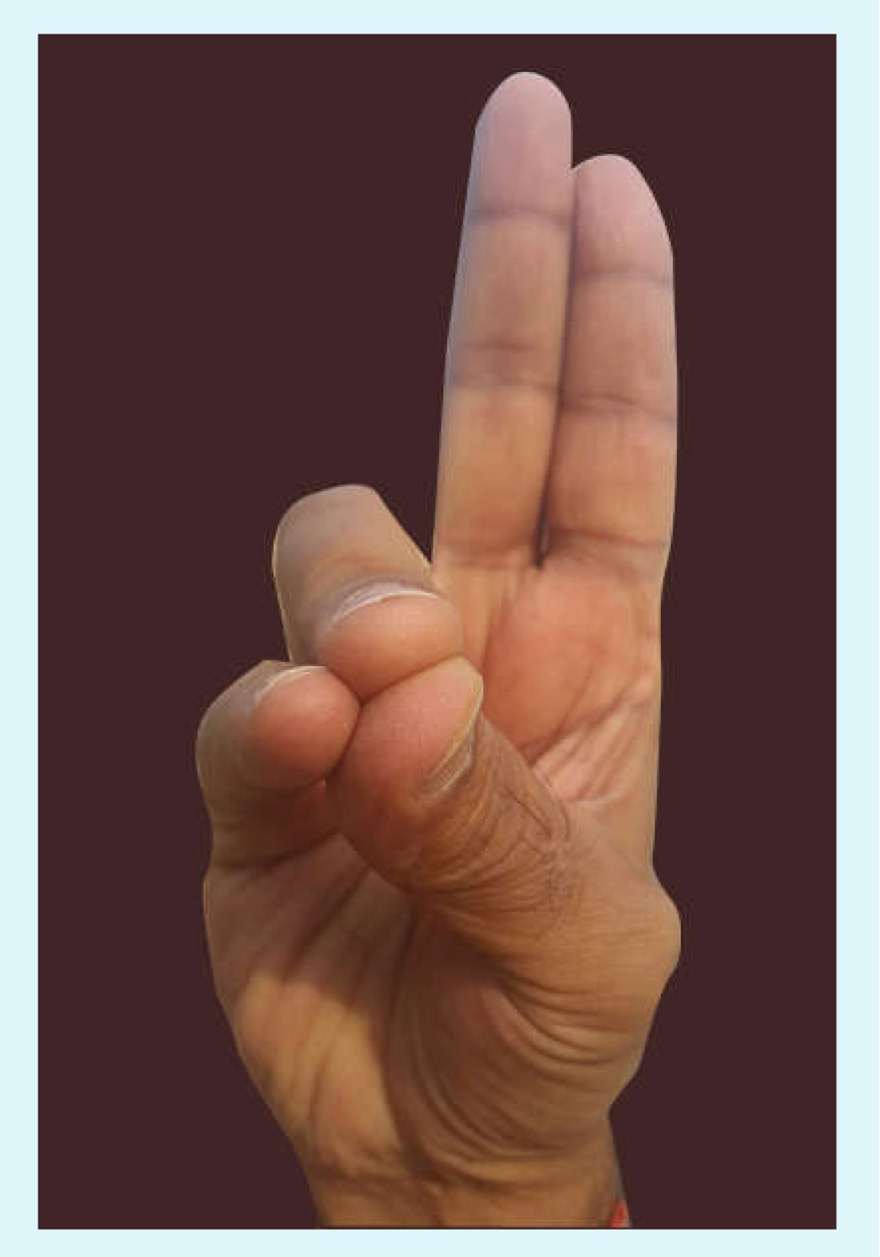
\includegraphics[width=0.4\linewidth,keepaspectratio]{pranmudra}
		
		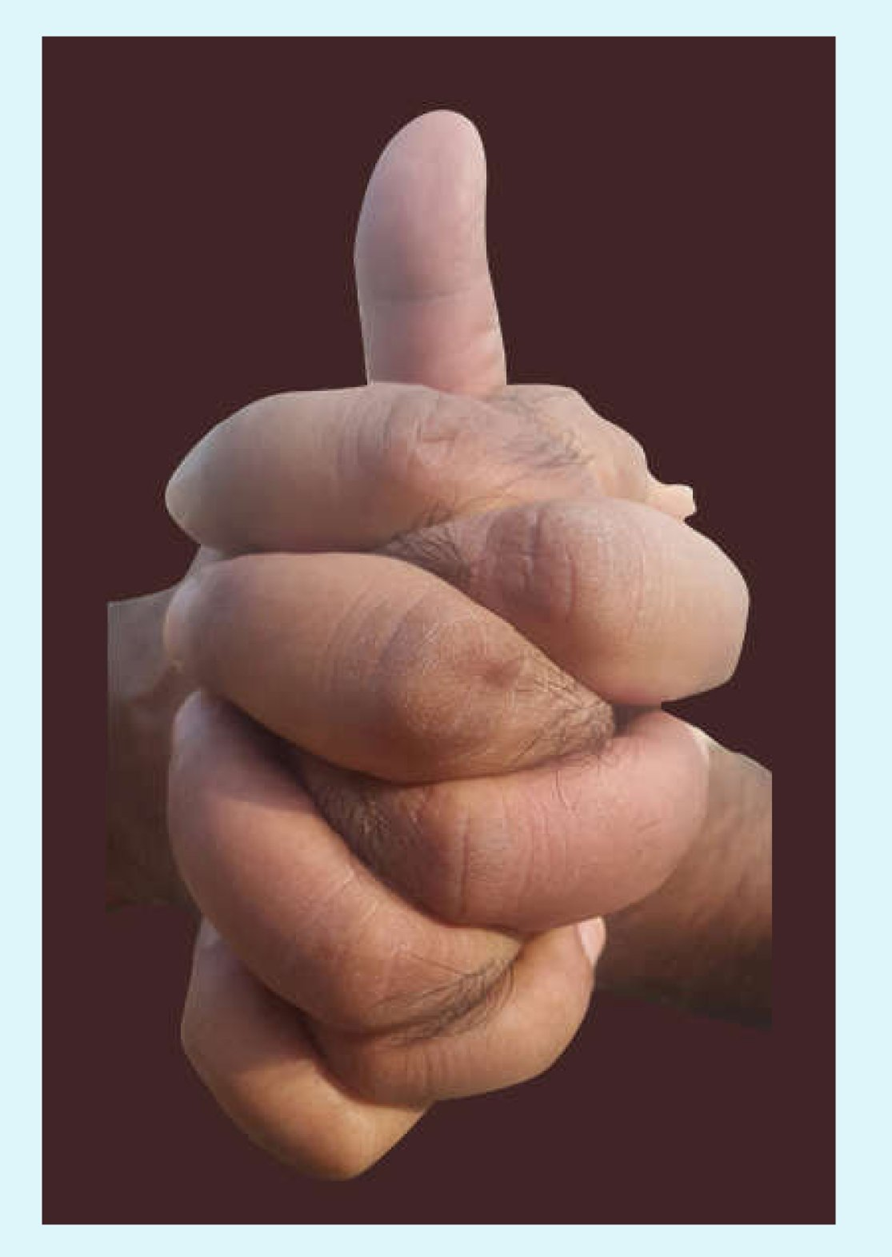
\includegraphics[width=0.4\linewidth,keepaspectratio]{lingmudra}
		
		\end{center}	
    \end{column}
  \end{columns}
  


{\tiny (Ref:  Building Immunity 2.0 - Shrimath Yoga)}

\end{frame}

%%%%%%%%%%%%%%%%%%%%%%%%%%%%%%%%%%%%%%%%%%%%%%%%%%%%%%%%%%%
\begin{frame}[fragile]\frametitle{Inner Silence}


		\begin{itemize}
		\item Part of Pratyahara (withdrawal of senses).
		\item Our attributes: We always seek to know, we wish to live forever and know what we dont know, even gossip is ok. We want to be happy.
		\item Level 1: learn to live with sensory pulls and pushes. Accept distractions. Going to retreat is running away from reality. We cannot change 'outside'. Be immune to it by being aware. Stand there in the problems. Be witness like a traffic police.
		\item Summary:
			\begin{itemize}
			\item Lesser thoughts
			\item Clarity in thought without confusion.
			\item Lack of prejudice and being open.
			\item Ability to stay calm even when triggered 
			\item Non judgmental and not jumping to conclusions even without listening and knowing about a subject.
			\end{itemize}
		\end{itemize}

  


{\tiny (Ref:  Master Class on Antar Mouna Level 1 - Shrimath Yoga)}

\end{frame}



